%!TEX root = ../main.tex

\section{Analysis} % (fold)
\label{sec:analysis}

In this chapter we will look into the advantages and disadvantages of sonification. 
Some of the advantages to consider are mentioned in the previous chapter, and so the advantages in this chapter will mainly be regarding using sound to convey data. 
We will also look into different contradicting terms in relation to sonification. 
Lastly, we look further into the sonification techniques that are available to us. 
This is so we can delimit what techniques we are to use when presenting data during our test. 
The advantages and disadvantages are so we know what to look out for in this regard. 

\FloatBarrier
\subsection{Advantages and Disadvantages of Sonification} % (fold)
\label{sub:advantages_and_disadvantages_of_sonification}

There are several advantages for sonification. Not only can it represent data and learn patterns and cycles in said data, but it can also aid the disabled and assist workers in different fields with sound patterns and alarms (Section~\ref{sec:preanalysis}).
However, as with everything there are certain disadvantages of sonification. 
The disadvantages can all be lead from the same disadvantages that sound has. Sound can be frustrating or annoying for some users, as people are forced to impose their own taste and ideas subjectively on data. 
Sound is also incredibly hard to describe in certain cases, you cannot mimic sound or make others interpret data without them being able to hear it. 
Listening to sound representing data can require learning or inherent talent, and this learning can take a longer time than looking at visually represented data, although that depends on the type of data. 
The type of data represented also needs to be taken into account for whenever a sound or pattern is chosen. 
\enquote{It is hard to represent a spatial arrangement with sound. You need to use the appropriate display.} Said Bruce Walker, a professor in the schools of psychology and interactive computing at Georgia Tech, running a group called the sonification lab \cite[Sec. Opportunities and pitfalls]{Feder2012}.
To give a more concrete example of an advantage, sonification was used to study a model of an artificial heart pump, where a modulated sound was indicating pressure on a pusher plate, and a tapping sound indicated a blood cell entering threshold vorticity, and a drum indicated the opening and closing of heart valves. 
It was reported that it seemed easier to determine different things, such as the frequency of blood cells crossing and detecting whether or not the heart valves were opening or closing. 
This is in contrast to the standard method of looking at change in color on a monitor. 
Another example is sonification used to indicate seismic events caused by the fracturing of rock walls during a 3 month dig. 
The engineers had a visualization to indicate these fractures, but the events were short and to address this, they added a short sound that varied in volume depending on the magnitude of the event. 
The sounds would draw more attention to periods with more seismic activity, making it easier to detect overlapping events that indicate higher risk. 
Sounds are extremely useful when variables do not appear together in the same image, or require shifting visual attention from monitor to monitor. 
From these two examples, it is clear that when dealing with data that has a variety of events or over longer periods of time, using sound can make the data easier to comprehend.

With examples of advantages and disadvantages in the representation of data through sonification, and how it is used, it is also valid to research existing types of sonification that represent weather data. 
This will give indications towards pre existing solutions to sonification of weather data, and might enlighten plausible methods of how we should develop a prototype.


\subsubsection{Weather data represented using sound} % (fold)
\label{ssub:weather_data_represented_using_sound}

Engineers use visualizations to represent a large amount of data over complex systems, an auditory display can be useful in these cases, where the interpretant needs to keep his eyes focused on the visual data while also receiving data from an audio source. 
The quality and completeness of a fluid flow simulation was analyzed by comparing the sonified audio data generated by a simulated turbine and an actual recording of a turbine~\cite[Ch. 2]{Barrass1999}.
Sounds can make it easier to perceive cycles and rhythm, and also abnormalities in a large amount of data. 
Another example of a visualization designed by Simon Kravis at the CSIRO was made to assist the engineers planning a water treatment, works by using a computer model. 
Chemical concentrations in the river’s water are shown by various colored segments, according to the downpour over a one year period. 
They realized that it is difficult to watch the downpour graph and the river visualization at the same time, so they decided to add sonification to represent the downpour so that an engineer may pay less visual attention to the river, while quantities of the downpour are represented by rain-like sound. 
The result of this was that after several repetitions, an engineer could learn the patterns of the rainfall over the year and can anticipate cycles in downpour or dryness. 
The sound representation is meant to bind the different sets of visualizations together and make it easier to remember, and an engineer was able to make relations between chemicals that are never seen at the same time~\cite{Barrass1998}.

% subsubsection weather_data_represented_using_sound (end)

% subsection advantages_and_disadvantages_of_sonification (end)

\FloatBarrier
\subsection{Analogic vs Symbolic representation} % (fold)
\label{sub:analogic_vs_symbolic_representation}

There are many different ways to go about designing something that uses sonification. Methods for designing auditory displays have been classified along a spectrum between analogic and symbolic by Kramer~\cite*{Barrass1999}.
\enquote{An analogic representation is one in which there is an immediate and intrinsic correspondence between the sort of structure being represented and the representation medium.}
Meaning, there is one to one mapping between points in the data and points in representation space~\cite*{Barrass1999}. 
Examples for this include a Geiger counter or an auditory thermometer.

Its counterpart, symbolic representation, categorically denotes the thing being represented and relations within the representation do not necessarily reflect intrinsic relationships in what is being represented. 
Examples of a display like this are computer beeps, cell phone alarms and vehicle control notifications.

% subsection analogic_vs_symbolic_representation (end)

\FloatBarrier
\subsection{Semiosis} % (fold)
\label{sub:semiosis}

Semiotics is the study of signs and their creation and interpretation. 
Signs can be anything from images to words, sounds and smells. 
These signs have no inherent meaning other than the one we attribute to them. 
Modern semiotics is based on the work of two major figures, Ferdinand de Saussure and Charles Sanders Peirce, a Swiss linguist and an American scientist respectively~\cite*{Vickers2012}.
In Saussure’s view the sign system is a dyadic relationship between a \enquote{signifier} and a \enquote{signified}.
A signifier is typically a sound pattern, and a signified is the meaning that signifier carries. 
An example of this is the symbol \texttt{/cat/}, which in this case is a signifier for the concept or meaning that we know as a cat. 
The link evoked between the sound pattern and the meaning is the resultant sign. 
Peirce considered this relationship to be insufficient, and he proposed another scheme in which an object referred to is represented by a \enquote{representamen} which then evokes in the mind of the listener the meaning of the sign which he refers to as the \enquote{interpretant}. 
The two theories loosely refer to one another and can be shown as such~\cite*{Vickers2012}(Figure~\ref{fig:semiosis1}):

\begin{figure}[!htbp]
    \centering
    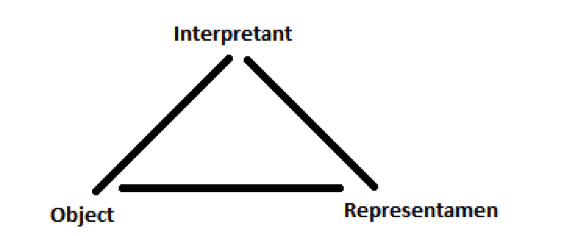
\includegraphics[width=.5\textwidth]{images/Semiosis1.png}
    \caption{Semiosis}
    \label{fig:semiosis1}
\end{figure}

% subsection semiosis (end)

\FloatBarrier
\subsection{Sonification usage} % (fold)
\label{sub:sonification_usage}

Sonification can be split up in 4 different kinds of function types, when going by theory created by Bruce N. Walker and Michael A. Ness~\cite*{walker2011}. 
The 4 different types are as follows: 

\begin{enumerate}
    \item Alarms, alerts, and warnings
    \item Status, process, and monitoring messages
    \item Data exploration
    \item Art and entertainment
\end{enumerate}


\paragraph{Alerting functions} % (fold)
\label{par:alerting_functions}
Alerting functions refers to sound indicating that a certain event is occurring or has occurred, but it usually won’t convey descriptive data on the alerted subject. 
For example, a microwave oven makes a beep when the timer has expired, but it will not tell you if the containing substance is done or overcooked. 
Another example is the usage of calendar notifications on phones or tablets. 
These notifications will only notify you that something is going to happen by ringing or beeping. 
To further understand what the occurring sound means, a visual clue or a memory of the upcoming event is required.

The last example in this category is a fire alarm. 
A fire alarm will ring loudly to alert you that you need to move immediately, in most cases out of the building, but it does not contain any information about the location of the fire, nor does it tell you how severe the fire is.

% paragraph alerting_functions (end)


\paragraph{Status and progress functions} % (fold)
\label{par:status_and_progress_functions}

Status and progress function has a purpose similar to that of alerting functions, but to understand the data correctly, a visual display or another form of continuous data is required to fully understand the situation at hand. 
It requires the interpretant to pay attention to small changes in the auditory feedback. 
This relates to the example given (Section~\ref{ssub:examples_of_sonification}) that we have previously discussed, where surgeons focus their eyes on the patient while listening to the heart monitors.

When designing a weather application, this could be the function to use if your goal was to have mostly visual data, only supplied by auditory data. 
However, it is important to note that when using this type of sonification, the auditory display itself is only a sub part of the data. 

% paragraph status_and_progress_functions (end)


\paragraph{Data exploration functions} % (fold)
\label{par:data_exploration_functions}

When talking of sonification, this is the function usually referred to. 
Data exploration is meant to encode and convey information about entire sets of data, or relevant aspects of said data.
Sonification designed for data exploration is different from status or process indicators, seeing as they use sound to offer a more \enquote{holistic portrait} of the data, as opposed to condensing information to capture a momentary state~\cite*{walker2011}.

% paragraph data_exploration_functions (end)


\paragraph{Art and Entertainment} % (fold)
\label{par:art_and_entertainment}

Since the sound producing capabilities of computers have evolved exponentially over the past years, so have the music producing of computers too. 
Sound data like sonification have been adapted more and more in to the world of music, and more artist uses data mapping included in their song or tracks. 
Since music does not really convey any form of information, it can still be included in the sonification functions, since it still conveys the expression/data of art and entertainment.

% paragraph art_and_entertainment (end)

The above covers the different sonification functions, and in which cases they can be useful to alert or notify interpretants.

The above covers the different sonification functions, and in which cases they can be useful to alert or notify interpretants.
As stated above, sonification has a lot of functioning abilities regarding how you can use audification without speech to notify a user what happens around them without using their eyes or hands, but sonification can also be categorized in their techniques and how you approach them. 
So far we have only explained what sonification can be used for, but not how the techniques are in practice, does it require interaction from a user or not?

Those approaches can be categorized in 3 categories which are (1) event based, (2) Model Based (3) Continuous.


\paragraph{Event-based sonification} % (fold)
\label{par:event_based_sonification}

The Event based approach is where the data of the sonification display is employed by the parameter mapping. 
Parameter mapping are changes in data dimension with changes in an acoustic dimension to produce a sonification. 
Parameter sees changes in data and then try to convey that data with as much as a feasible display through sounds, to show what that data means, a lot like what we want to do with data of the weather. 
The event based approaches have more or less through time, had a passive interaction possibility with brief notification like alarms and notification, but event based sonification that employ parameter mapping have the possibility to adapt to both passive and active interaction.

The sonification Handbook~\cite[Ch. 15]{Hermann2011} shows several examples of sound that tells the user e.g. that their target destination is reached.
The data will read the remaining length of the journey and then intensify the sonification/sound depending on how close you are to your target.

% paragraph event_based_sonification (end)


\paragraph{Model-based sonification} % (fold)
\label{par:analysis_model_based_sonification}

Model based differs from event based a lot, since here you need a virtual model that relies heavily on the interaction between the user and the virtual object. 
The virtual object then reads the users interaction, and converts that interaction into sonification. 

The Sonification Handbook video number 16.3~\cite*[Ch. 16, Vid. 16.3]{Hermann2011} shows a perfect example of model based sonification. 
You see a user with a triangular object moving around, the software then detects his movement and convert his actions in to sounds depending on how the object is moved. 
Another example of this can be a metal detector, which some people uses on the beach to scavenge forgotten objects on the beach. 
The metal detector will notify/alarm you if your metal detector senses any metal beneath its reader. 

% paragraph analysis_model_based_sonification (end)


\paragraph{Continuous sonification} % (fold)
\label{par:continuous_sonification}

Continuous sonification is possible when data are timed series and sampled at a rate that a quasi-analog signal can be directly translated in to sound (quasi-analog signal in telecommunication is a digital signal that has been converted to a suitable form for transmission through analog channel). 
To explain it more simply is when sound waves are directly translated in to sound. 
That means the conversion happens when the software translates the data from a sound wave into sound e.g. a Richter scale converts seismic data in to wave forms. 
The wave forms are displayed with an accuracy of 90\%.

% paragraph continuous_sonification (end)


We will generally focus on the first category of sonification, but not in the sense that we need to alarm people.
We know that sonification can notify you in many different ways. 
Some forms require a passive listener and some requires and active listener, maybe both. 
The approaches for sonification are also different depending on the task or the message you wish to convey. 
We also know that sonification can have interaction methods that require the user to physically interact with an object to generate sonification to work. 
According to our research regarding sonified weather data, it is stated that engineers needed to become familiar with the sound to know the intensity of the rain. 
We will therefore expect that if the users are hearing the sound for the first time, they may not give the correct answer.

% subsection sonification_usage (end)


For the prototype we will be using event based sonification. 
Continious sonification could also be used, if we were to take weather data and directly transform it into sonification, but this will not be the case in the prototype. 
The type we will be using is data exploration, since we wish to translate weather data into sounds that can be heard by the end user during testing.
Using event based sonification means we will employ parameter mapping. 
Theoretically this would mean that we have the ability to change the sound as our weather data changes, which seems to be the ideal choice.
So to summarize what we have learned and what we will use in our prototype, we will dive right into a list of requirements.

% section analysis (end)
